\item A continuación, se muestran tres representaciones posibles (figuras \ref{fig:2i-a}, \ref{fig:2i-b} y \ref{fig:2i-c}) referidas a las relaciones entre \textbf{Sitios de taxis}, \textbf{Choferes} y \textbf{Taxis}. Analiza las ventajas y desventajas de cada propuesta, contestando las preguntas que se presentan a continuación:

\begin{figure}[H]
	\centering
	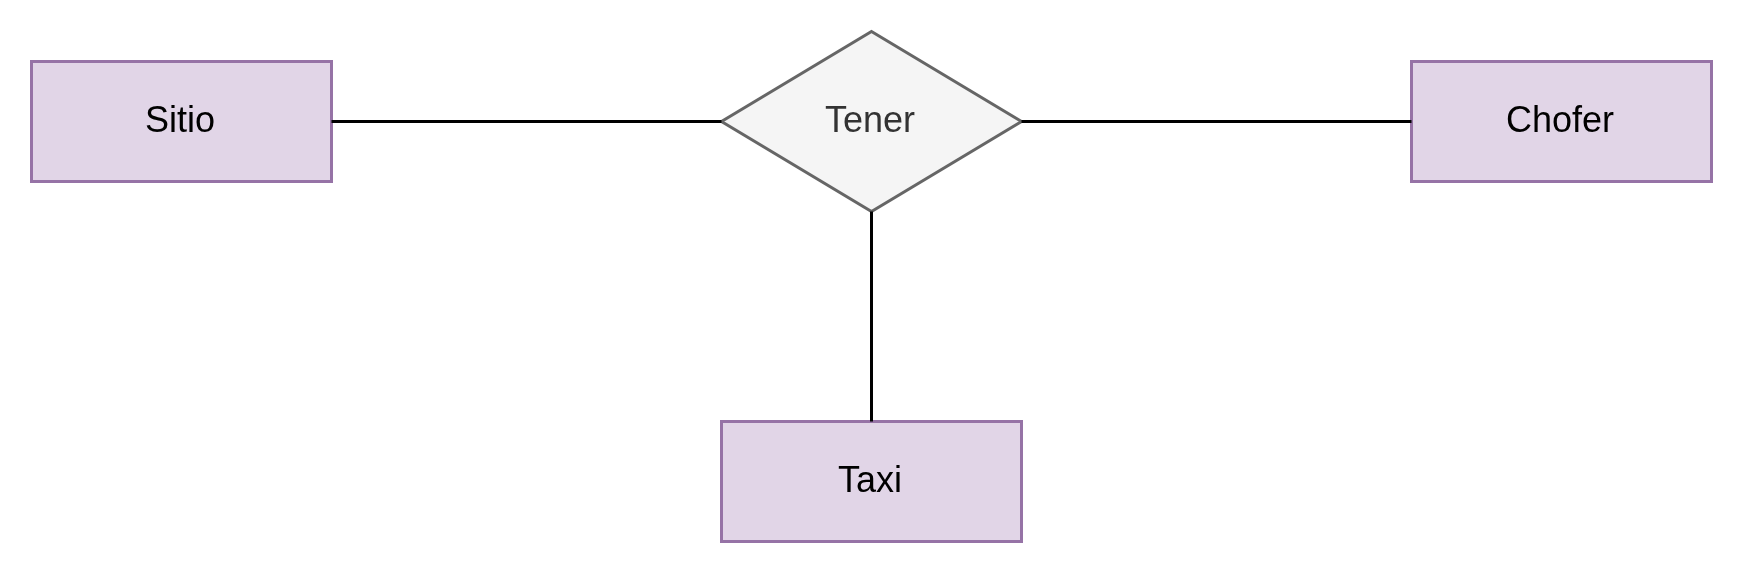
\includegraphics[width=0.62\textwidth]{Figuras/ejercicio2i_a.png}
	\caption{Representación a) de las relaciones entre Sitios, Choferes y Taxis.}
	\label{fig:2i-a}
\end{figure}

\begin{figure}[H]
	\centering
	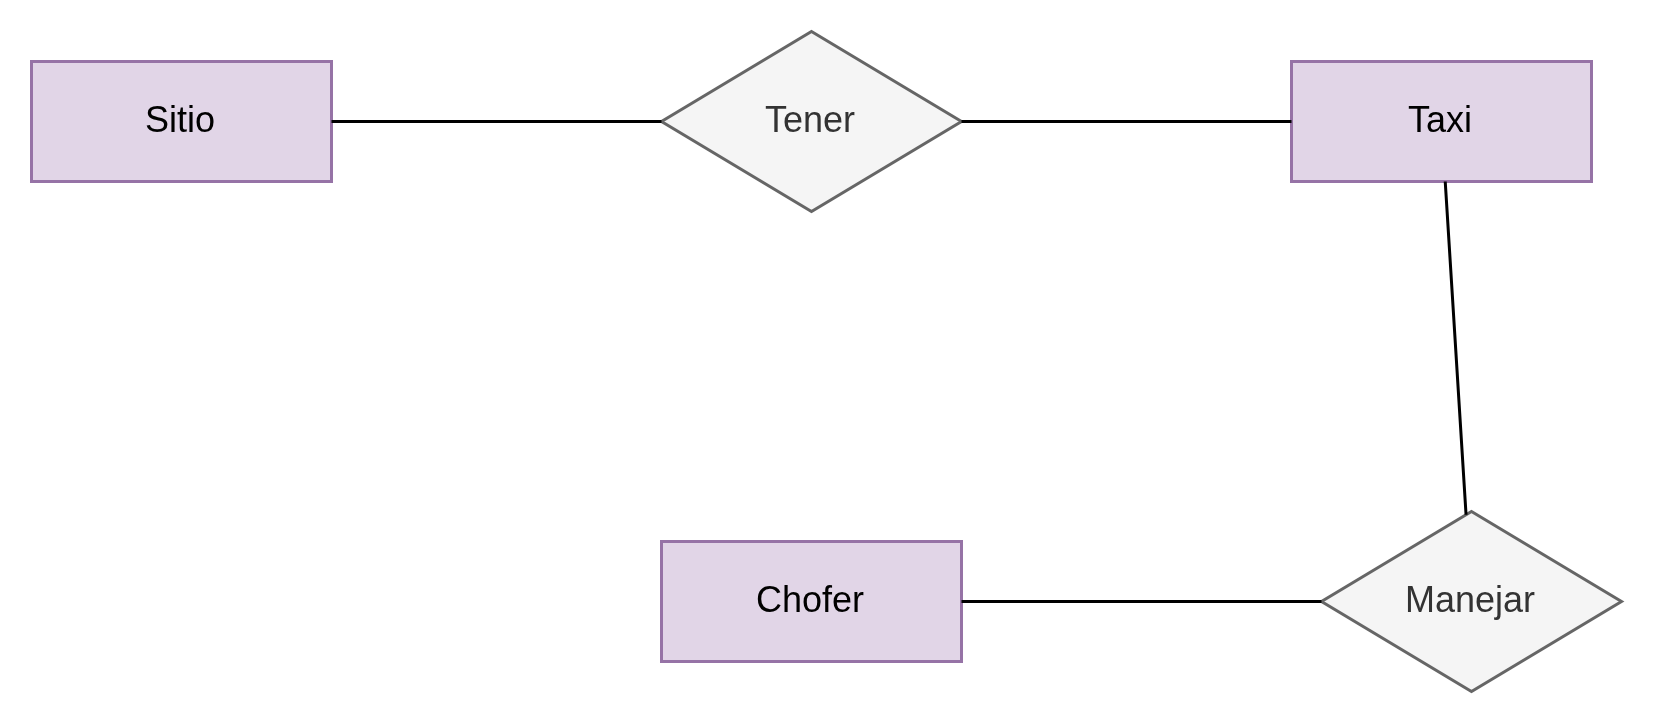
\includegraphics[width=0.95\textwidth]{Figuras/ejercicio2i_b.png}
	\caption{Representación b) de las relaciones entre Sitios, Choferes y Taxis.}
	\label{fig:2i-b}
\end{figure}

\begin{figure}[H]
	\centering
	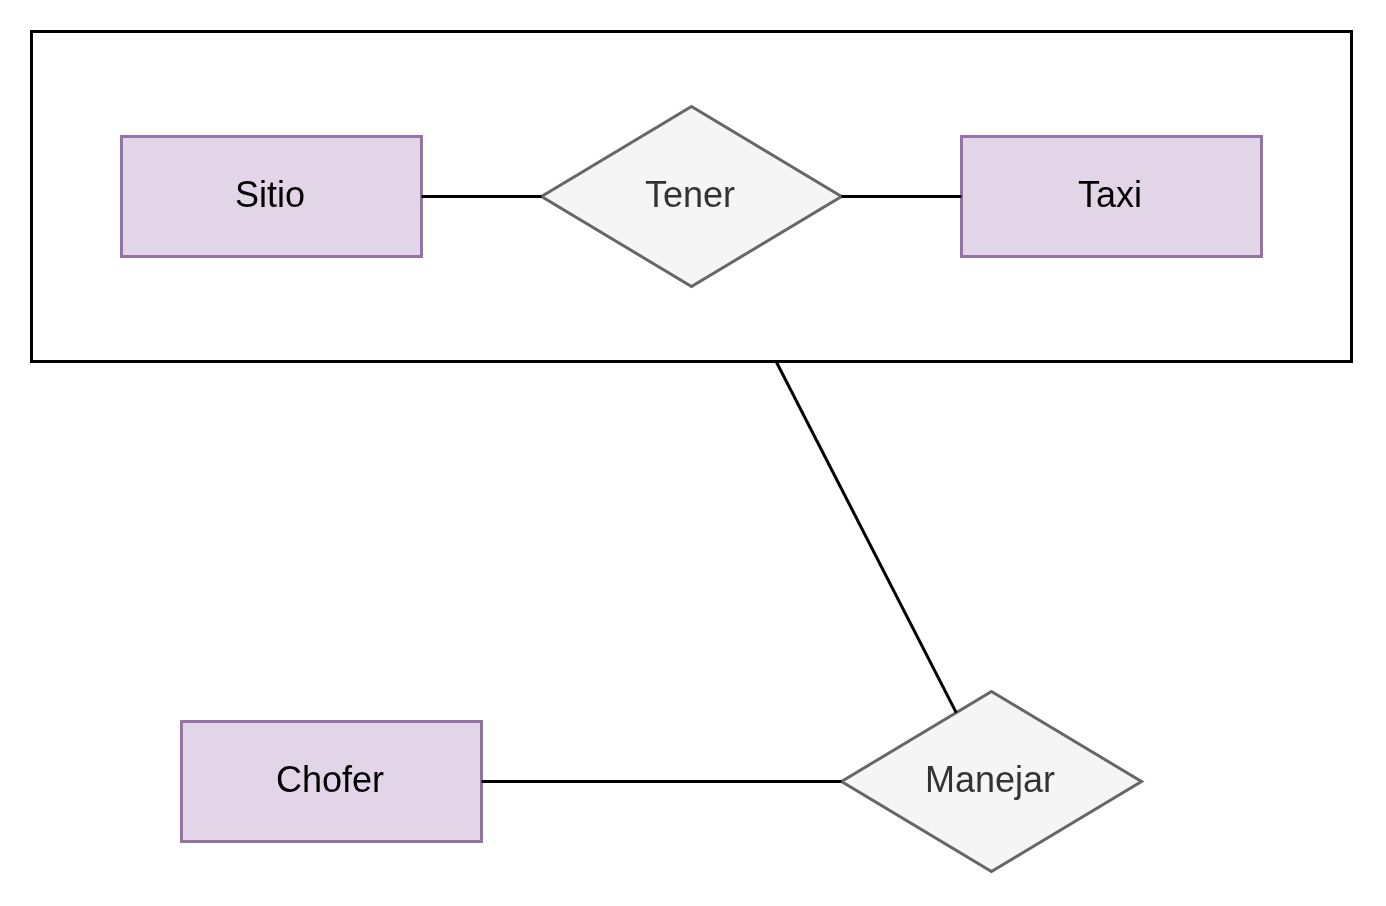
\includegraphics[width=0.72\textwidth]{Figuras/ejercicio2i_c.png}
	\caption{Representación c) de las relaciones entre Sitios, Choferes y Taxis.}
	\label{fig:2i-c}
\end{figure}

\begin{itemize}
	\item \textbf{Indica qué diagramas representan la información requerida por las siguientes solicitudes de información:}

	\textbf{¿Qué taxis maneja el chofer Raúl López en el sitio Santa Fe?}

	Solo los diagramas a) y c) dejan responder esto. Ambos capturan en una relación el hecho de que un chofer maneja un taxi específico en un sitio específico (a) mediante una relación ternaria y c) mediante la combinación de Tener con Manejar), por lo que se puede filtrar directamente por chofer y sitio para obtener el taxi. En el diagrama b), Manejar sólo relaciona Chofer con Taxi, sin ninguna referencia al sitio, así que no podemos saber en qué sitio maneja Raúl López un taxi específico (básicamente la situación que sale en errores comunes en las notas).

	\textbf{¿A qué sitios está afiliado el chofer Carlos Reyes?}

	De nuevo, solo a) y c) lo permiten, ya que en ambos el chofer queda relacionado al sitio con una misma relación. En b) el chofer solo se relaciona con los taxis que maneja, y el sitio se obtiene por separado a través de Tener(Sitio, Taxi) y como no hay garantía de que el chofer maneje ese taxi específicamente en ese sitio (el taxi podría estar en ese sitio en otro momento o con otro chofer), no se puede inferir que un chofer pertenece a un sitio.

	\textbf{¿Qué taxis están asociados al sitio Universidad?}

	Esta pregunta la responden los tres diagramas, en todos existe una relación (directa en b y c, por proyección en a) entre Sitio y Taxi que no depende del chofer.

	\item \textbf{¿Qué modificación harías en el diagrama de la figura \ref{fig:2i-a}, sin perder información, para que se puedan conocer qué taxis que maneja cada chofer?}

	Agregaría una relación binaria adicional \textit{Maneja} directamente entre Chofer y Taxi, independiente de la relación \textit{Tener}. De esta forma, conservamos toda la información original (qué chofer maneja qué taxi en qué sitio usando \textit{Tener}) y se puede consultar directamente qué taxis maneja un chofer sin importar el sitio.

	\begin{figure}[H]
		\centering
		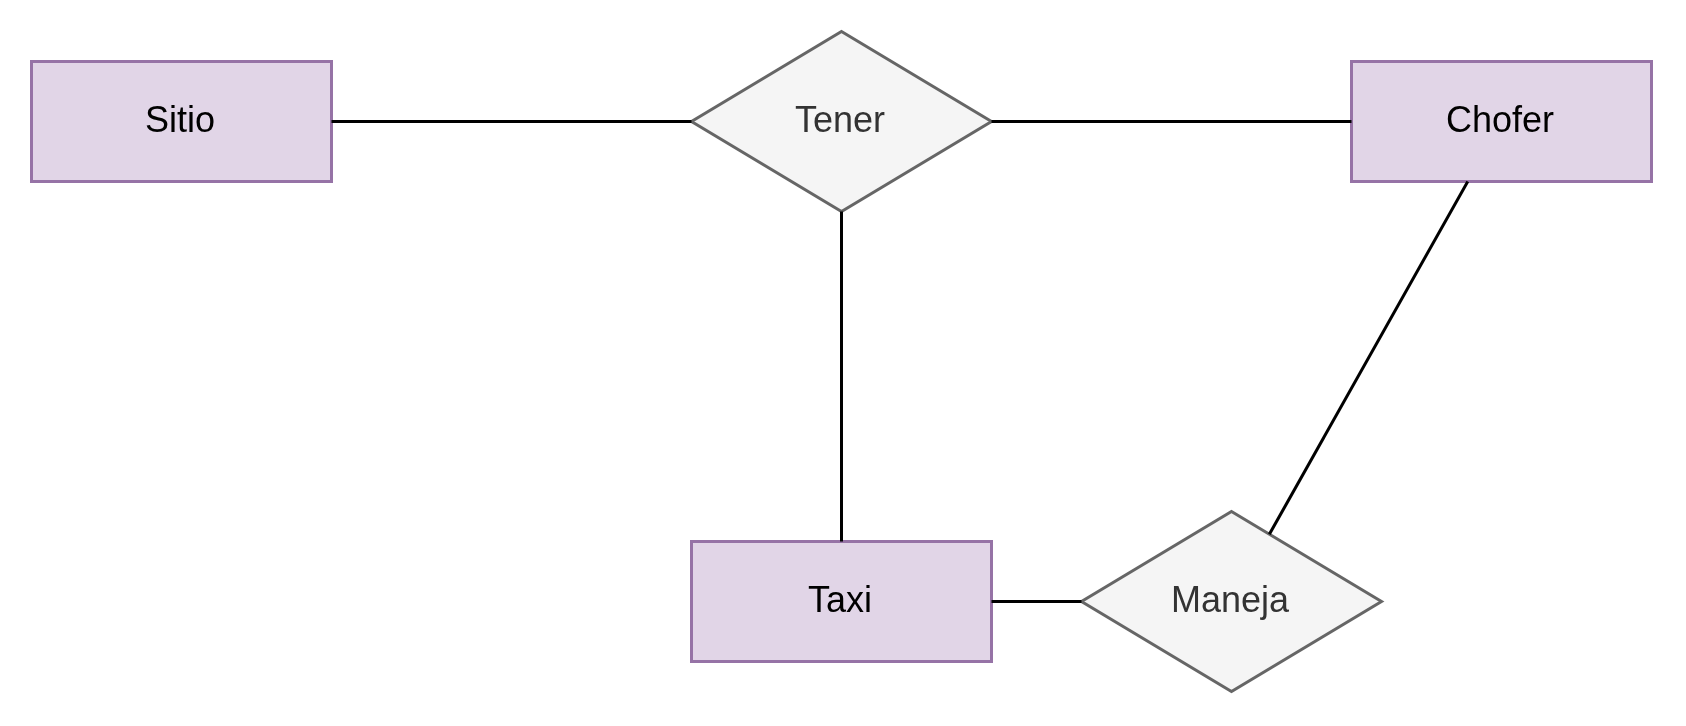
\includegraphics[width=0.8\textwidth]{Figuras/2i_modificado.png}
		\caption{Diagrama propuesto a partir de la figura \ref{fig:2i-a}, agregando la relación binaria \textit{Maneja} entre Chofer y Taxi.}
		\label{fig:2i-maneja}
	\end{figure}

	\item \textbf{¿Qué diferencia existe entre los diagramas de las figuras \ref{fig:2i-a} y \ref{fig:2i-c}?}

	Ambos diagramas terminan representando la misma información (qué chofer maneja qué taxi en qué sitio), pero lo hacen de forma distinta. En a) se usa una sola relación de grado tres (ternaria) que conecta Sitio, Chofer y Taxi. En c) se usa una agregación, primero se define la relación binaria \textit{Tener} entre Sitio y Taxi y después esa relación completa se trata como si fuera una entidad para relacionarla usando \textit{Manejar} con Chofer. en otras palabras, c) descompone en dos pasos binarios lo que a) resuelve en un paso, pero ambos preservan la combinación de los tres elementos a la vez, a diferencia de b).

	\item \textbf{Cómo modificarías el diagrama de la figura \ref{fig:2i-a} para representar las siguientes restricciones:}

	\textbf{Un chofer no puede manejar más de un taxi en el mismo sitio.}

	Se agregaría una restricción de cardinalidad sobre la relación ternaria \textit{Tener}, colocando un 1 del lado de Taxi. Esto se interpreta como que, para cada combinación de (Sitio, Chofer), existe a lo más un Taxi asociado.

	\textbf{Un taxi no puede ser manejado por más de un chofer en el mismo sitio.}

	De manera análoga, se coloca un 1 del lado de Chofer, para indicar que por cada combinación de (Sitio, Taxi) existe a lo más un Chofer asociado.

	\begin{figure}[H]
		\centering
		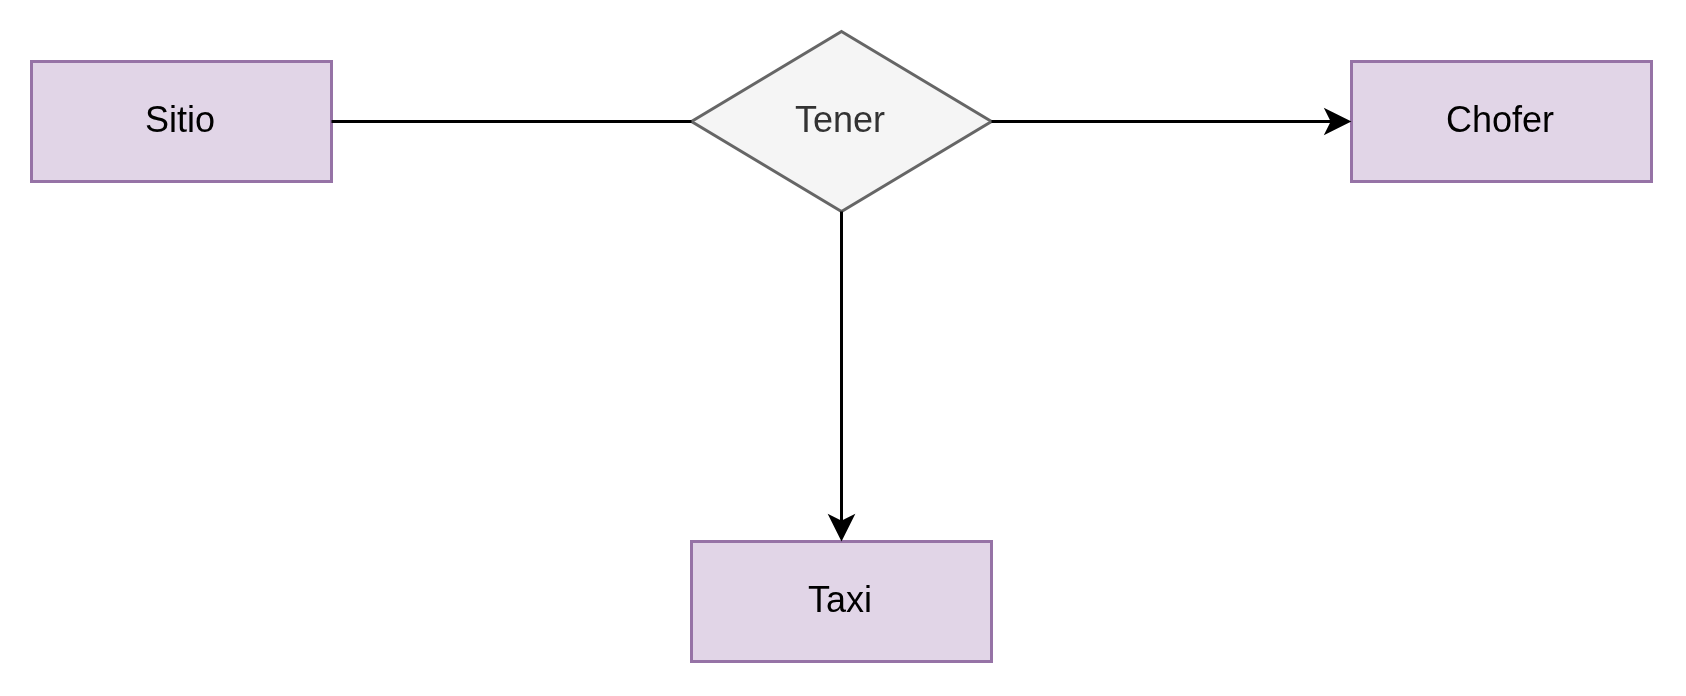
\includegraphics[width=0.8\textwidth]{Figuras/2i_restricciones.png}
		\caption{Diagrama de la figura \ref{fig:2i-a} con las restricciones de cardinalidad (\textbf{1}) en los lados de \textit{Chofer} y \textit{Taxi}.}
		\label{fig:2i-restr}
	\end{figure}
\end{itemize}

\textbf{Nuevo modelo propuesto}

Tomamos como base el diagrama \ref{fig:2i-a}, incorporamos el modelo modificado y queda de la siguiente forma:

Entidades: Sitio, Chofer y Taxi, cada una con sus atributos correspondientes (p.~ej. Sitio con su nombre como identificador, Chofer con su número de licencia como identificador, Taxi con su placa como identificador).

Relación ternaria \textit{Tener} entre Sitio, Chofer y Taxi, con las restricciones de cardinalidad 1 del lado de Taxi como del lado de Chofer, lo que expresa que un chofer no puede manejar más de un taxi en el mismo sitio y que un taxi no puede ser manejado por más de un chofer en el mismo sitio.

En cuestión de participación, Sitio participa de forma parcial en \textit{Tener} (puede haber sitios sin choferes ni taxis registrados todavía), mientras que Chofer y Taxi participarían de forma total, un chofer o un taxi sólo tiene sentido en el sistema si está asociado a al menos un sitio.

Finalmente, se conserva la relación binaria \textit{Maneja} entre Chofer y Taxi del punto anterior, para poder consultar directamente qué taxis maneja cada chofer sin tener que pasar por el sitio.

\begin{figure}[H]
	\centering
	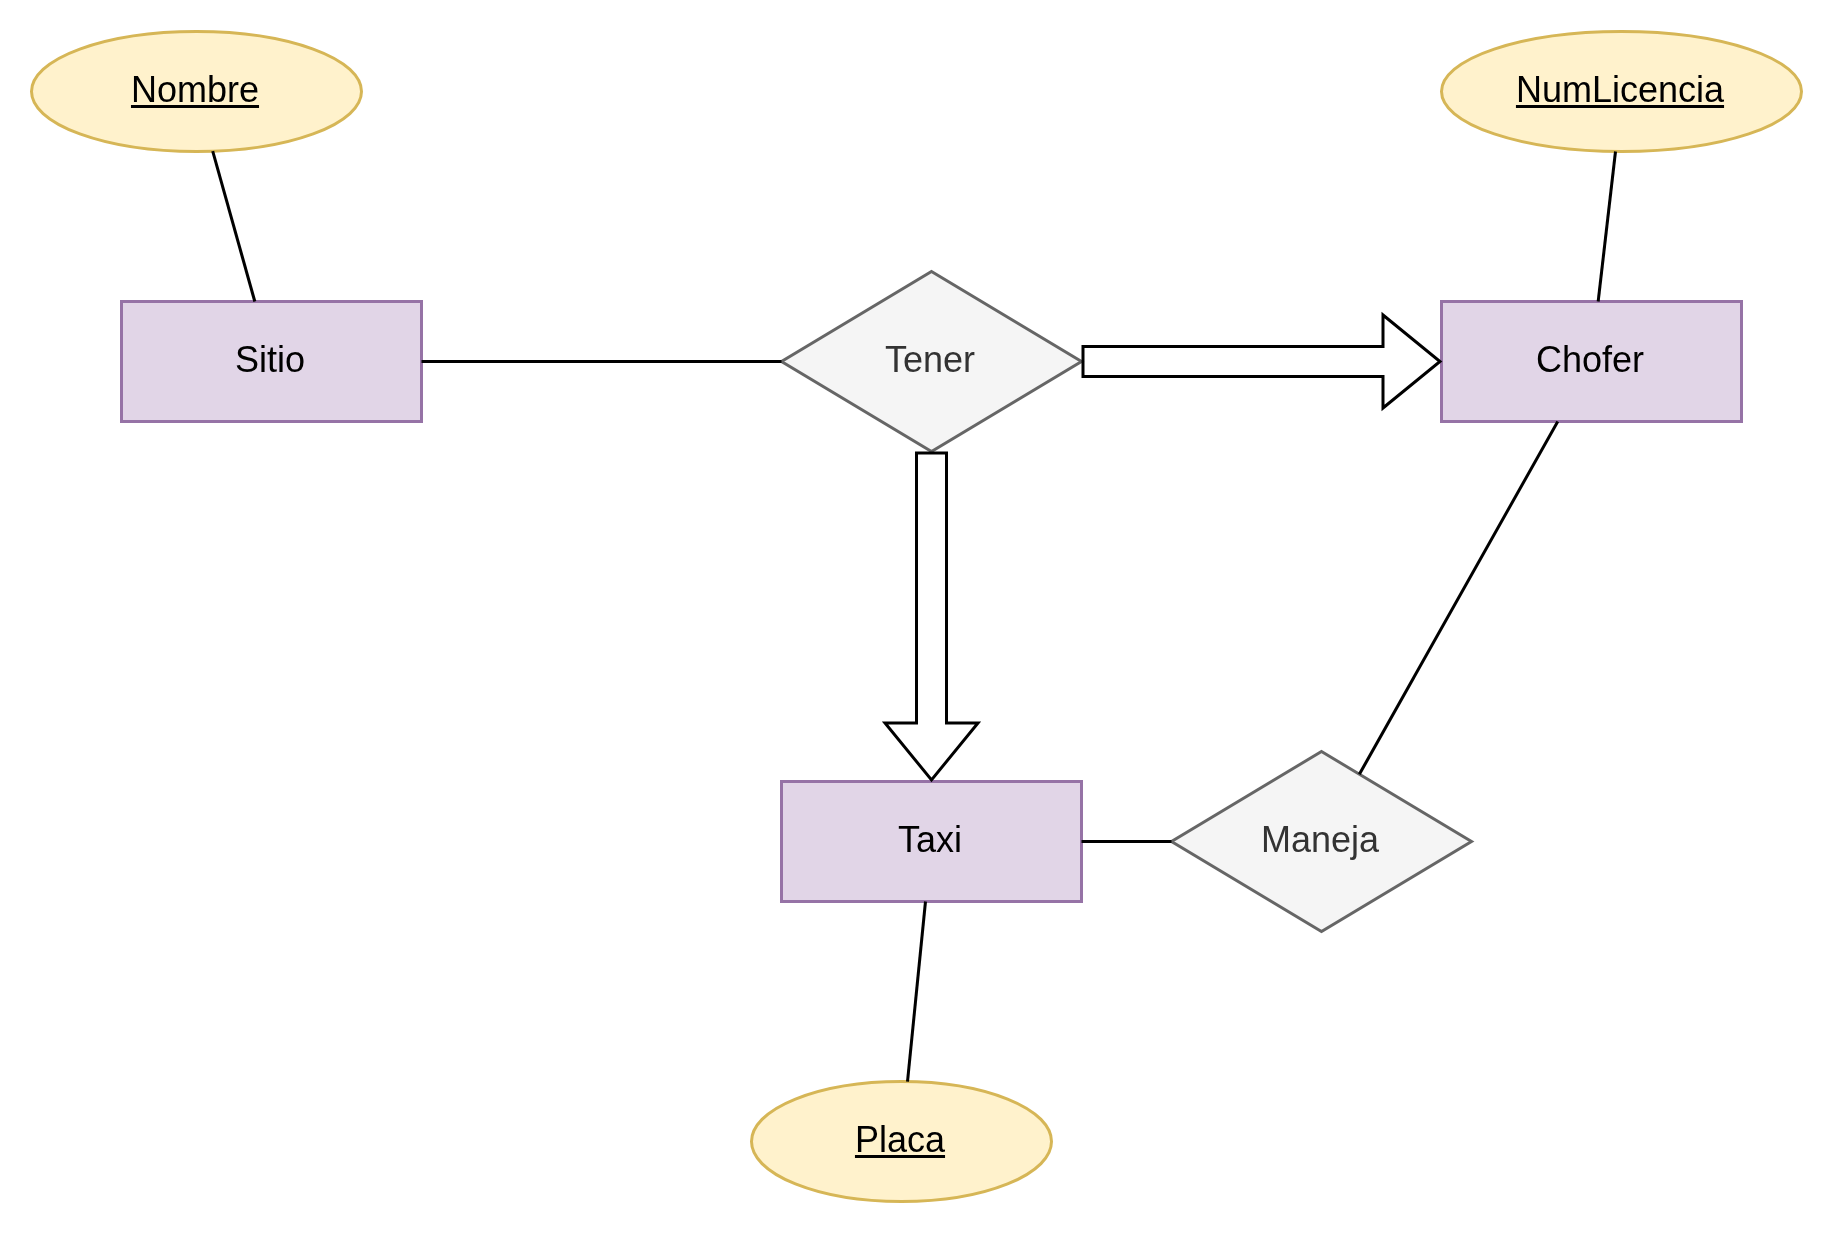
\includegraphics[width=0.85\textwidth]{Figuras/2i_modelo.png}
	\caption{Modelo E-R propuesto para el problema de los sitios de taxis, con las restricciones de cardinalidad y participación.}
	\label{fig:2i-modelo}
\end{figure}
